
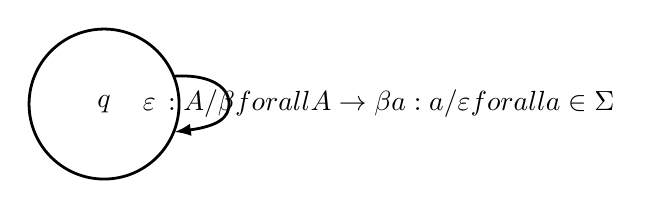
\begin{tikzpicture}[>=latex,line join=bevel,]
  \pgfsetlinewidth{1bp}
%%
\pgfsetcolor{black}
  % Edge: q -> q
  \draw [->] (52.443bp,37.036bp) .. controls (63.028bp,37.728bp) and (72bp,34.383bp)  .. (72bp,27bp) .. controls (72bp,22.155bp) and (68.136bp,19.049bp)  .. (52.443bp,16.964bp);
  \definecolor{strokecol}{rgb}{0.0,0.0,0.0};
  \pgfsetstrokecolor{strokecol}
  \draw (125bp,27bp) node {$ \begin{matrix} \varepsilon: A/\beta \text{ for all } A \to \beta \\ a: a/\varepsilon \text{ for all } a \in \Sigma \\ \end{matrix}$};
  % Node: q
\begin{scope}
  \definecolor{strokecol}{rgb}{0.0,0.0,0.0};
  \pgfsetstrokecolor{strokecol}
  \draw (27bp,27bp) ellipse (27bp and 27bp);
  \draw (27bp,27bp) node {$q$};
\end{scope}
%
\end{tikzpicture}

